
\section{Ethernet 2 (Ethernet Systeme)}

\subsection{Virtuelle LANs}

\paragraph{Trunk-Links} Trunk Links sind Teil von mehreren VLANs. Auf den Trunk Links müssen Frames der verschiedenen VLANs eindeutig gekennzeichnet werden!

\paragraph{VLAN-Tag} Erweiterung des Ethernet Headers durch einen
VLAN-Tag.
Die maximalen Nutzdatenlänge bleibt erhalten,
der Ethernet Frame wird 4 Bytes länger
{
\begin{itemize}[noitemsep]
    \item Type 0x8100 $\to$ getaggtes Frame
    \item Priority Code Point ermöglicht die Priorisierung gewisser Applikationen
    \item Discard Eligibility Indicator 0 → Frame wird bei Überlastsituationen zuerst verworfen
    \item VLAN Tagging erfolgt oft beim Eintritt / Austritt ins Netz
    \item  Für Endgeräte unsichtbar
\end{itemize}
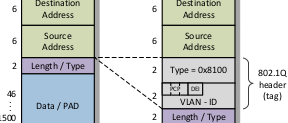
\includegraphics[scale=.75]{img/vlan.png}
\WhiteSpace
}

\subsection{Spanning Tree}

{\paragraph{Ziel:}  Alle Segmente in einer loop-freien Topologie verbinden}
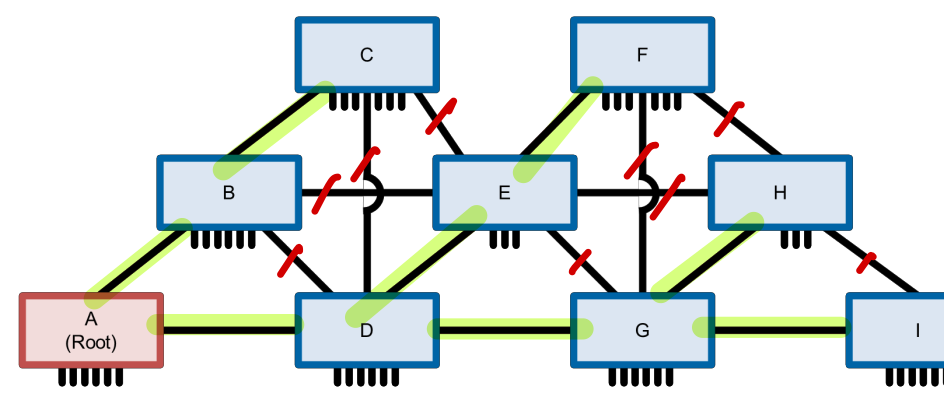
\includegraphics[scale=.275]{img/spanning_tree.png}

\subsection{Autonegotiation}

{\paragraph{Ziel:}  Ermittlung der besten Betriebsart durch Austausch der
    Leistungsmerkmale zweier Netzwerkkomponenten.}

\subsection{Bridges}

\subsection{Router}

\subsection{ARP (Address Resolution Protocol)
}


